\documentclass{standalone}
\usepackage{tikz}
\usetikzlibrary{shapes}
\usepackage{tikzpeople}

\begin{document}

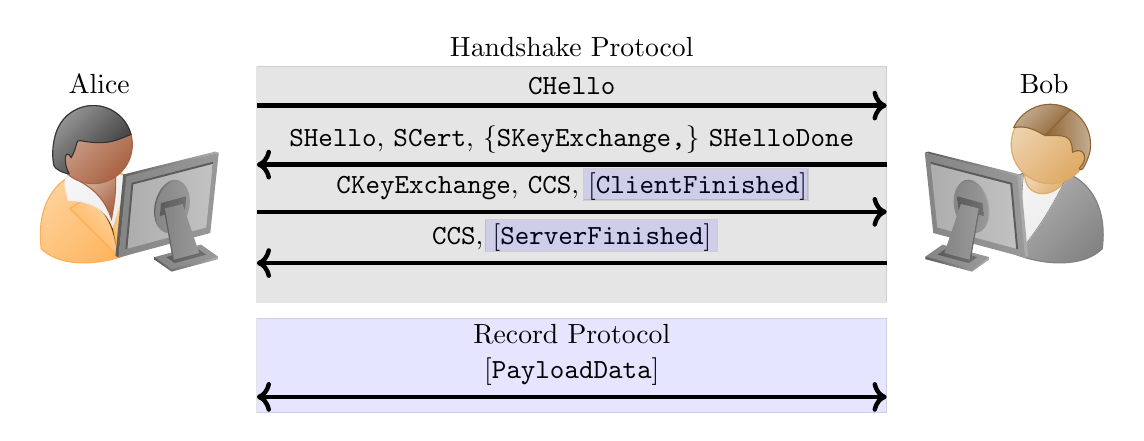
\begin{tikzpicture}
\tikzset{
	cylinder/.style={draw,
		shape=cylinder,
		name=nodename, % Can be defined arbitrarily
		alias=cyl, % Will be used by the ellipse to reference the cylinder
		aspect=1.5,
		minimum height=8.5cm,
		minimum width=2.25cm,
		color=blue,
		fill= blue!30,
		outer sep=-0.5\pgflinewidth, % to make sure the ellipse does not draw over the lines
		%shape border rotate=90
}}

\draw[draw=black,fill=black, opacity=0.1] (2,4) rectangle  (10,1);
\draw[draw=black,fill=blue, opacity=0.1] (2,0.8) rectangle  (10,-0.4);
\node[] (HSKLBL) at (6,4.25) {Handshake Protocol};
\node[] (HSKLBL) at (6,0.6) {Record Protocol};
\node[alice, monitor, label=Alice, minimum size=1.5cm] (Alice) at (0,2.5) {};
\node[bob, mirrored, monitor, label=Bob, minimum size=1.5cm] (Bob) at (12,2.5) {};

{\draw[->, ultra thick] (2,3.5)  -- (10,3.5) node[midway, above] {\texttt{CHello}};}
{\draw[<-, ultra thick] (2,2.75)  -- (10,2.75) node[midway, above] {\texttt{SHello}, \texttt{SCert}, \{\texttt{SKeyExchange,}\} \texttt{SHelloDone}};}
{\draw[->, ultra thick] (2,2.15)  -- (10,2.15) node[midway, above] {\texttt{CKeyExchange}, \texttt{CCS}, [\texttt{ClientFinished}]};}
{\draw[draw=black,fill=blue, opacity=0.1] (6.15,2.7) rectangle  (9,2.3);}
{\draw[<-, ultra thick] (2,1.5)  -- (10,1.5) node[midway, above] {\texttt{CCS}, [\texttt{ServerFinished}]};}
{
	\draw[draw=black,fill=blue, opacity=0.1] (4.9,2.05) rectangle  (7.85,1.65);}
{\draw[<->, ultra thick] (2,-0.2)  -- (10,-0.2) node[midway, above] {[\texttt{PayloadData}]};}
\end{tikzpicture}

\end{document}
